\subsection{Q10.14 data 10312021 grouped by scenario \& PGM}

\begin{comment}
                             EFPR        EO      EFNR     n    pvalue
(frauth, Advantaged)     0.400000  0.600000  0.350000  20.0  0.232414
(frauth, Disadvantaged)  0.000000  1.000000  1.000000   1.0  1.000000
(icu, Advantaged)        0.650000  0.350000  0.600000  10.0  0.157299
(icu, Disadvantaged)     0.333333  0.666667  0.388889   9.0  0.180207
(rent, Advantaged)       0.062500  0.937500  0.187500   8.0  0.012419
(rent, Disadvantaged)    0.538462  0.461538  0.461538  13.0  0.630760
\end{comment}

\begin{table}[h]
    \centering
    \begin{tabular}{|c|c|c|c|c|c|c|}
        \hline
        scenario & PGM & EFPR & EO & EFNR & n & p-value\\
        \hline
        frauth & Advantaged & 0.400 & \textbf{0.600} & 0.350 & 20.0 & 0.232\\
		frauth & Disadvantaged & 0.000 & \textbf{1.000} & \textbf{1.000} & 1.0 & 1.000\\
		icu & Advantaged & \textbf{0.650} & 0.350 & \textbf{0.600} & 10.0 & 0.157\\
		icu & Disadvantaged & 0.333 & \textbf{0.667} & 0.389 & 9.0 & 0.180\\
		rent & Advantaged & 0.062 & \textbf{0.938} & 0.188 & 8.0 & \textbf{0.012}\\
		rent & Disadvantaged & \textbf{0.538} & 0.462 & 0.462 & 13.0 & 0.631\\
		
        \hline
    \end{tabular}
    \caption{Grouped by scenario PGM}
    \label{tab:my_label}
\end{table}
\begin{figure}[h]
    \centering
    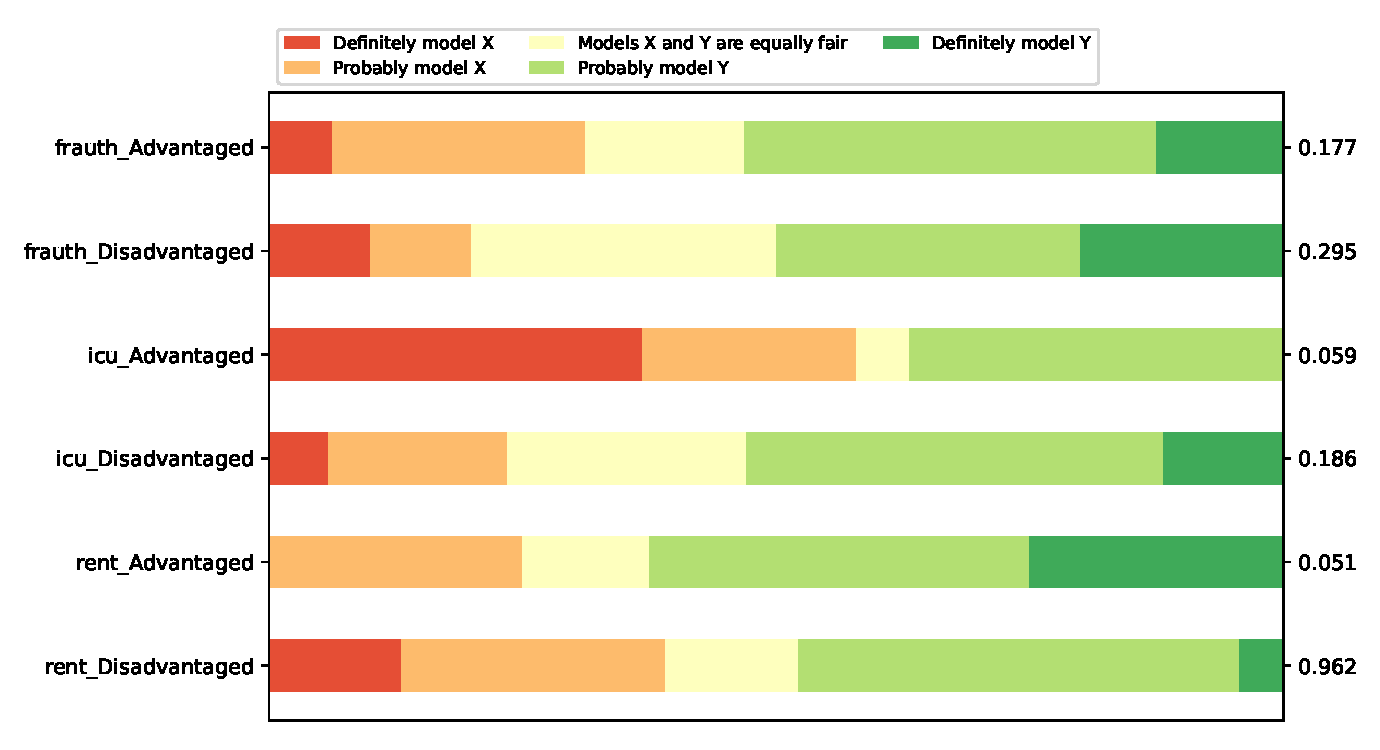
\includegraphics[width=0.8\textwidth]{figures/Q10.14/10312021/Q10.14_scenario_PGM.pdf}
    \caption{Grouped by scenario \& PGM}
    \label{fig:my_label}
\end{figure}
